\section{Results}
\label{sec:results}

\subsection{Synthetic Sensitivity Results}
\label{subsec:synthetic-results}

Table~\ref{tab:failure-modes} and the extended sweep results in
Sections~\ref{subsec:motivation-results}--\ref{subsec:apls-recovery} are this section's synthetic
eval-metric results, computed directly against the live library for this paper rather than reused
from prior notes.

\subsection{Real-Data Case Studies}
\label{subsec:realdata-results}

\begin{itemize}
  \item \textbf{Finding \#1 --- DTAF1 blind spot, confirmed on real data.} Averaged across 24 real
    SpaceNet tiles (Vegas + Khartoum), 75\% road-pixel dropout leaves plain DTAF1 at
    $\mathbf{1.000}$ while CBHM collapses to $\mathbf{{\sim}0.57}$ (driven by
    \texttt{cldice\_mean} falling to ${\sim}0.40$). \texttt{dtaf1\_weighted} does \textbf{not} fix
    this --- also stays at 1.000, since area-weighting only changes how per-class scores combine,
    not the per-pixel tolerance-matching logic within a class. \textbf{Open item}:
    \texttt{dtaf1\_topo} has not yet been re-validated on this real 24-tile sample
    (synthetic-only so far, Section~\ref{subsec:dtaf1topo}) --- flagged as future work
    (Sections~\ref{sec:discussion}--\ref{sec:conclusion}).
  \item \textbf{Finding \#2 --- CBHM sparse-class collapse, \texttt{Khartoum\_img371} case study.}
    Detailed in Section~\ref{subsec:weighted-reduction}: 12px road offset $\to \mathrm{cbhm}=0.000$
    vs.\ $\mathrm{dtaf1}=0.934$; \texttt{cbhm\_soft} recovers only to $\mathbf{0.285}$ because the
    road has more GT pixels than the building despite its tiny area share.
  \item \textbf{Contrast case (\texttt{Khartoum\_img333})}: $\mathrm{cbhm}$ $0.48$--$0.52 \to
    \mathrm{cbhm\_soft}$ $\mathbf{0.85}$ --- a clean win where the building genuinely dominates by
    pixel count.
  \item \textbf{Aggregate table} across all 24 tiles: \texttt{road\_offset}@16px
    ($\mathrm{cbhm}\ 0.669 \to \mathrm{cbhm\_soft}\ 0.712$), \texttt{road\_dropout}@0.75
    ($\mathrm{cbhm}\ 0.568 \to \mathrm{cbhm\_soft}\ 0.646$).
  \item \textbf{Point-feature results} on 15 Potsdam crops: \texttt{point\_dropout} (precision
    flat at 1.000, recall falls linearly to 0), \texttt{point\_clutter} (recall flat at 1.000,
    precision $1.0 \to 0.36 \to 0.13$ at 5/20 spurious blobs), \texttt{point\_jitter} (drops to
    ${\sim}0.38$ by 6px on real data --- faster than the synthetic sweep, attributed to real
    objects being packed closer together).
\end{itemize}

\subsection{Applied Pipeline: Trained U-Net Results (CE+Dice Baseline)}
\label{subsec:unet-results}

\begin{table}
  \caption{Full test-set table (15 held-out tiles, mean $\pm$ std).}
  \label{tab:unet-baseline}
  \begin{tabular}{@{}lcc@{}}
    \toprule
    Metric & mean & std \\
    \midrule
    \texttt{cbhm} & 0.316 & 0.126 \\
    \texttt{cbhm\_soft} & 0.378 & 0.130 \\
    \texttt{dtaf1} & 0.440 & 0.134 \\
    \texttt{dtaf1\_weighted} & 0.476 & 0.141 \\
    \texttt{cldice\_mean} & 0.409 & 0.193 \\
    \texttt{bf\_mean} & 0.308 & 0.156 \\
    \bottomrule
  \end{tabular}
\end{table}

Best tile \texttt{Shanghai\_img1375} ($\mathrm{cbhm}=0.617$), worst \texttt{Shanghai\_img1711}
($\mathrm{cbhm}=0.163$). Framed explicitly as ``first end-to-end validation that the metric
library scores an actual trained model's output sensibly,'' not as a SOTA benchmark claim. This
table is the CE+Dice \textbf{baseline} side of Section~\ref{subsec:joint-results}'s forthcoming
ablation.

\subsection{Loss Ablation Results}
\label{subsec:lossablation-results}

Seven sweeps (Section~\ref{subsec:lossablation-setup}) confirm the qualitative story
Table~\ref{tab:correspondence} predicts --- each new loss term responds distinctly to the
perturbation family its \texttt{metrics/} counterpart is designed to catch, and stays flat (a
negative control) under perturbations that don't touch its configured class(es). All values below
are each configuration's own raw loss value (not the cumulative \texttt{plus\_X} framing) at
representative severities, computed directly against the live code for this paper:

\textbf{Road offset sweep} (tolerance radius $=10$px): \texttt{tolerance}'s own value stays
essentially flat ($0.0043$) through offset $=10$px, then climbs ($0.0056$ at 12px) exactly at its
configured tolerance boundary --- reproducing the eval-side ``holds until exactly the tolerance
boundary'' story on the training-signal side. \texttt{cldice}'s own value jumps almost immediately
(already at $1.0$ loss delta by offset $=2$px) and then plateaus at its collapsed value ---
reproducing clDice's documented zero-tolerance-to-offset property.

\textbf{Road thickness sweep} (GT fixed 3px): \texttt{cldice}'s own value tracks the
\texttt{ce\_dice} baseline closely through thickness $=13$px (within ${\sim}0.05$ of each other at
every point up to a $4\times$ width ratio), then diverges sharply from thickness $=15$px onward ---
reproducing Section~\ref{subsec:cldice-loss}'s unit-test finding ($3\times$ ratio scores
identically to exact width) at a coarser, sweep-level granularity and confirming the
$\mathrm{iters}{=}10$ default's practical width-invariance range.

\textbf{Building erosion sweep}: \texttt{tolerance} tracks building erosion closely (a consistent
gap above \texttt{ce\_dice}, e.g.\ $1.2338$ vs.\ $1.0526$ at erosion radius $=11$px, reflecting the
tight 2px building tolerance), while \texttt{cldice} stays essentially identical to
\texttt{ce\_dice} throughout ($1.0531$ vs.\ $1.0526$) --- the expected negative control, since
\texttt{SoftClDiceLoss} is configured over linear classes only.

\textbf{Point jitter/dropout/clutter sweeps}: \texttt{heatmap} is by far the most shape-sensitive
term, rising from a baseline of $0.58$ to $70.6$ by 8px of jitter (then plateauing/slightly
declining as points scatter further from any plausible match) --- while \texttt{tolerance} and
\texttt{cldice} stay flat at their perturbation-independent baseline values throughout every point
sweep, confirming both as correct negative controls. \texttt{ce\_dice}'s own value also rises
modestly under point perturbations ($0.51 \to 0.84$ under jitter), but nowhere near as sharply or
as saturating as \texttt{heatmap}'s response.

\textbf{No flat curve was found where sensitivity was expected} --- every term's own raw value
moves under the perturbation family its \texttt{metrics/} counterpart is designed to catch, and
every intended negative control stayed flat. See \texttt{tests/test\_loss\_sensitivity.py}'s
module docstring for the full per-sweep numeric tables.

\subsection{Joint Multi-Source Training Results}
\label{subsec:joint-results}

\textbf{Executed} (\texttt{notebooks/train\_unet\_joint.ipynb}, this revision).
Section~\ref{subsec:joint-setup}'s setup ran to completion: 153 cached tiles loaded (123 SpaceNet
+ 30 Potsdam), split per-source 70/15/15 (SpaceNet: 86/18/19 train/val/test; Potsdam: 21/4/5),
patchified to 3117 train + 652 val patches. A per-batch source-mix printout confirmed both sources
appear in training (batches 0--2: 16/0, 16/0, 15/1 spacenet/potsdam patches) --- Potsdam patches
are necessarily rare per batch (only 21 of 3117 train patches, ${\approx}0.7\%$, since each
Potsdam crop contributes exactly one already-patch-sized tile versus 36 patches per large SpaceNet
tile), but they are not absent.

Training ran for 2 epochs (reduced from the baseline's 15 --- an explicit, stated scope choice for
this CPU-only pipeline sanity check, not a claim that more epochs wouldn't help):

\begin{table}
  \caption{Joint training: per-epoch total and sub-term losses.}
  \label{tab:joint-training}
  \begin{tabular}{@{}cccccc@{}}
    \toprule
    Epoch & train\_loss & val\_loss & ce\_dice & tolerance & cldice \\
    \midrule
    1 & 3.3824 & 2.8458 & 1.5427 & 0.5896 & 0.9038 \\
    2 & 2.6823 & 2.5957 & 1.2497 & 0.5509 & 0.8718 \\
    \bottomrule
  \end{tabular}
  \vspace{2pt}
  {\footnotesize heatmap: $0.3461 \to 0.0098$ (shown separately in Figure~\ref{fig:joint-subterms}
  for scale).}
\end{table}

\begin{figure}
  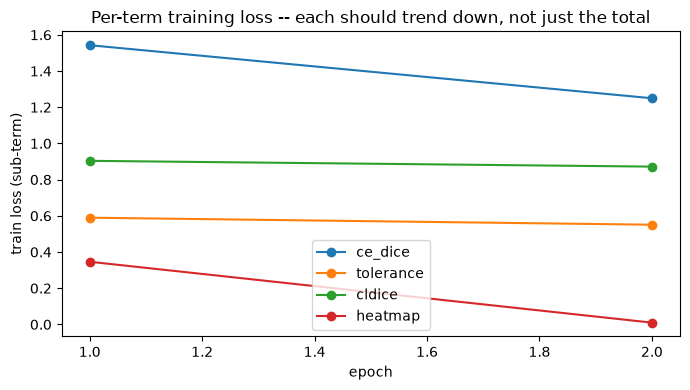
\includegraphics[width=\linewidth]{figures/joint_training_subterm_curves.png}
  \Description{Line chart of four per-term training loss curves (ce\_dice, tolerance, cldice,
  heatmap) over 2 epochs. All four lines slope downward; the heatmap curve drops most steeply,
  from about 0.35 to about 0.01.}
  \caption{Per-term training loss over 2 epochs --- all four sub-terms decrease, not just the
  total; \texttt{heatmap} drops most sharply (a $35\times$ reduction).}
  \label{fig:joint-subterms}
\end{figure}

\textbf{Verification passed}: all four sub-terms decreased epoch-over-epoch, not just the total
(Figure~\ref{fig:joint-subterms}) --- \texttt{heatmap} dropped the most sharply ($0.346 \to 0.010$,
a $35\times$ reduction), consistent with the model quickly learning that predicting near-zero
point probability almost everywhere is a strong early strategy given how sparse real point
coverage is even within Potsdam patches.

\begin{table}
  \caption{Joint model test-set evaluation, split by source, via \texttt{evaluate\_all()} with
  \texttt{point\_classes=[3]} and a 4-class \texttt{dtaf1\_config}.}
  \label{tab:joint-test}
  \begin{tabular}{@{}lcc@{}}
    \toprule
    Metric & SpaceNet-only ($n{=}19$) & Potsdam-only ($n{=}5$) \\
    \midrule
    \texttt{cbhm} & $0.144 \pm 0.115$ & $0.000 \pm 0.000$ \\
    \texttt{cbhm\_soft} & $0.230 \pm 0.119$ & $0.078 \pm 0.159$ \\
    \texttt{dtaf1} & $0.304 \pm 0.157$ & $0.092 \pm 0.149$ \\
    \texttt{dtaf1\_weighted} & $0.371 \pm 0.212$ & $0.076 \pm 0.158$ \\
    \texttt{cldice\_mean} & $0.173 \pm 0.141$ & $0.000 \pm 0.000$ \\
    \texttt{bf\_mean} & $0.252 \pm 0.151$ & $0.078 \pm 0.159$ \\
    \texttt{point\_f1\_mean} & --- & $0.200 \pm 0.447$ \\
    \bottomrule
  \end{tabular}
\end{table}

\textbf{Verification passed}: \texttt{point\_f1\_mean} is non-\texttt{None} for 5/5 real stitched
Potsdam test tiles (values $[0.0, 0.0, 0.0, 1.0, 0.0]$) --- the first time
\texttt{evaluate\_all()}'s \texttt{point\_classes} argument has ever been exercised end-to-end on
a real trained model's output, not left \texttt{None}.

\textbf{Baseline comparison}: the raw \texttt{data/train\_unet\_test\_results.csv} this session's
\texttt{train\_unet.ipynb} would produce was not present in this environment (that baseline was
originally run in an earlier session; only its already-documented aggregate survives,
Table~\ref{tab:unet-baseline}: \texttt{cbhm} $0.316\pm0.126$, \texttt{dtaf1} $0.440\pm0.134$, 15
epochs, single-source SpaceNet-only 3-class model), so no row-matched comparison was possible this
session --- only a directional one against those published aggregates. The joint run's
SpaceNet-only \texttt{cbhm} ($0.144$) and \texttt{dtaf1} ($0.304$) both come in \textbf{lower}
than the baseline's. Read this honestly rather than as evidence the new loss underperforms: this
run trained for 2 epochs against the baseline's 15, on a bigger effective task (a 4-class head
jointly absorbing gradient from four loss terms, one of them from a source, Potsdam, contributing
under 1\% of training patches) --- an apples-to-apples epoch-matched comparison has not been run.
\textbf{Framed honestly as a pipeline sanity check, not a benchmark or an ablation claim}, matching
Section~\ref{subsec:trainedmodel-setup}'s own posture toward the baseline itself.

\begin{figure}
  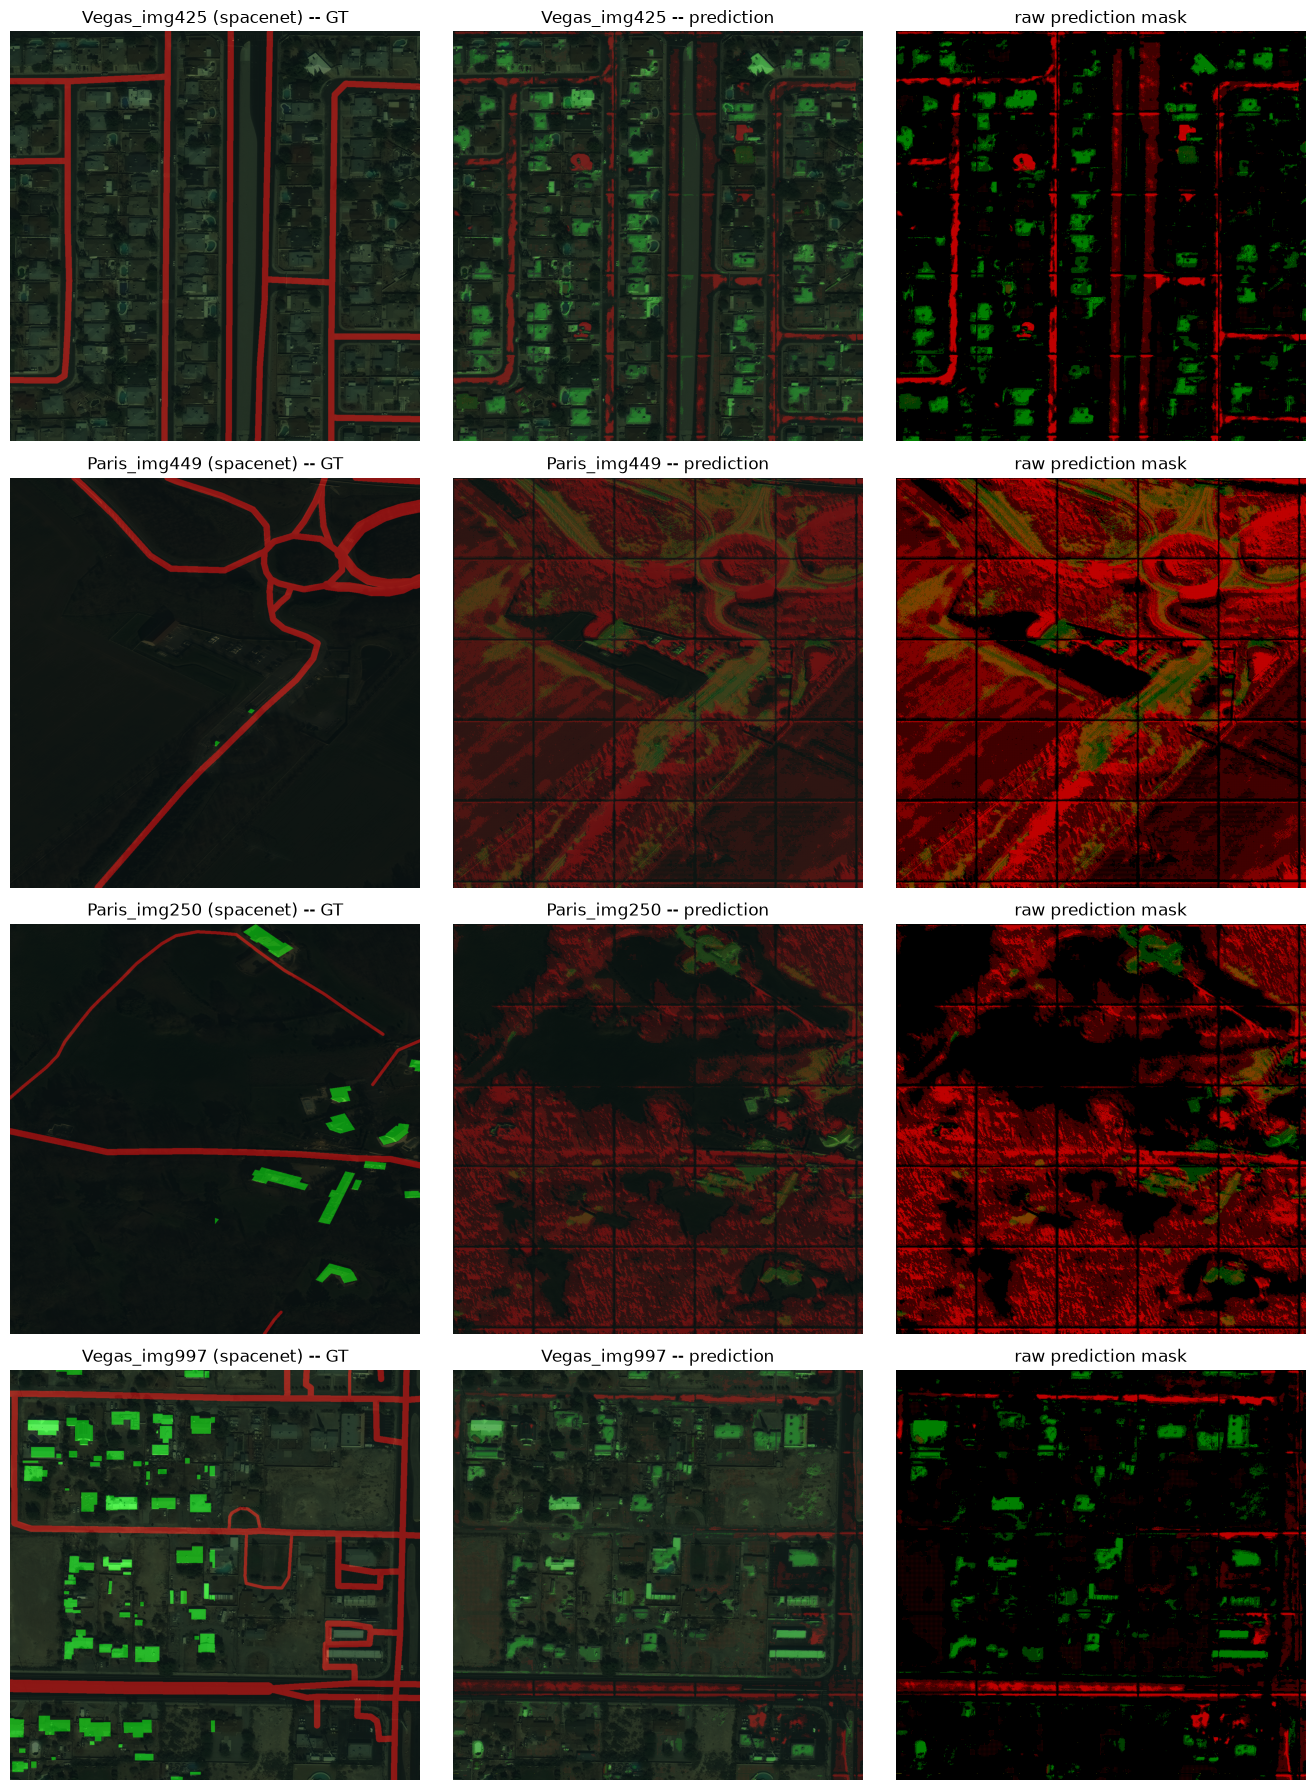
\includegraphics[width=\linewidth]{figures/joint_qualitative_panels.png}
  \Description{Four rows of three panels each (RGB image with GT overlay, RGB image with
  prediction overlay, raw prediction mask), one row per test tile, ordered worst to best by cbhm
  score: Vegas\_img425, Paris\_img449, Paris\_img250, Vegas\_img997. Roads are overlaid in red,
  buildings in green.}
  \caption{Qualitative review, worst$\to$best \texttt{cbhm} test tiles (GT / prediction / raw
  prediction mask; red$=$road, green$=$building). \texttt{Vegas\_img425} (top row, worst by
  \texttt{cbhm}) is visually one of the better-looking predictions --- see text for why its score
  is nonetheless exactly 0. \texttt{Paris\_img449}/\texttt{Paris\_img250} over-predict road across
  open terrain with no GT road, consistent with an underfit 2-epoch model.}
  \label{fig:joint-qualitative}
\end{figure}

\textbf{Qualitative review} (Figure~\ref{fig:joint-qualitative}, 4-color panels, worst$\to$best
\texttt{cbhm} tiles): mixed quality, as expected at 2 epochs, and one genuinely interesting
real-data finding. The \textbf{worst}-scoring tile by \texttt{cbhm} (\texttt{Vegas\_img425},
$\mathrm{cbhm}=0.000$) is visually one of the \emph{better}-looking predictions in the panel ---
road centerlines and building footprints are both recognizable and roughly aligned with GT. The
per-metric breakdown explains the apparent contradiction and is a real-data echo of
Section~\ref{subsec:cbhm}'s own ``harsh vs.\ lenient foil'' story: $\mathrm{bf\_mean}=0.000$
exactly (building Boundary F1, tolerance 2px, collapsed completely) while
$\mathrm{dtaf1\_weighted}=0.902$ and $\mathrm{cldice\_mean}=0.474$ are both high --- CBHM's
harmonic mean zero-collapses the \emph{entire} tile score from one class's tight-tolerance metric
hitting exactly zero, even though the lenient, tolerance-based DTAF1 view and the road-only clDice
view both say this tile is mostly correct. This is the first time that exact zero-collapse
mechanism (Appendix~\ref{app:a3}) has been observed on a real trained model's output rather than
only in synthetic scenes (Table~\ref{tab:failure-modes}) or GT-vs-perturbed-GT sweeps
(Section~\ref{subsec:realdata-results}). The best-scoring shown tile (\texttt{Vegas\_img997},
$\mathrm{cbhm}=0.364$) has a more balanced per-metric profile ($\mathrm{dtaf1}=0.402$,
$\mathrm{cldice\_mean}=0.336$, $\mathrm{bf\_mean}=0.397$) --- no single class collapsing, road and
building both partially but not perfectly recovered. The two weakest-looking predictions in the
panel (\texttt{Paris\_img449}, \texttt{Paris\_img250}) show substantial over-prediction of the
road class across open/agricultural terrain that has no GT road, consistent with an underfit
model at this epoch budget, not a structural failure of the joint loss or masking scheme. No
qualitative evidence of a masking bug (e.g.\ a SpaceNet tile hallucinating point-class
predictions, which would indicate \texttt{class\_mask} leaking) was observed in any reviewed
panel.
